\section{Methodology}
\label{sec:metho}
\subsection{Overview}
As shown in Fig.~\ref{fig:net}, given a sparse point cloud $\mathcal{P}\in\mathbb{R}^{N\times3}$, our proposed PU-Transformer can generate a dense point cloud $\mathcal{S}\in\mathbb{R}^{rN\times3}$, where $r$ denotes the upsampling scale. Firstly, the PU-Transformer head extracts a preliminary feature map from the input. Then, based on the extracted feature map and the inherent 3D coordinates, the PU-Transformer body gradually encodes a more comprehensive feature map via the cascaded Transformer Encoders. Finally, in the PU-Transformer tail, we use the shuffle operation~\cite{shi2016real} to form a dense feature map and reconstruct the 3D coordinates of $\mathcal{S}$ via an MLP.

In Alg.~\ref{alg:put}, we present the basic operations that are employed to build our PU-Transformer. As well as the operations (\enquote{MLP}~\cite{qi2017pointnet}, \enquote{Norm}~\cite{ba2016layer}, \enquote{Shuffle}~\cite{shi2016real}) that have been widely used in image and point cloud analysis, we propose two novel blocks targeting a transformer-based point cloud upsampling model \ie, the Positional Fusion block (\enquote{\textbf{PosFus}} in Alg.~\ref{alg:put}), and the Shifted-Channel Multi-head Self-Attention block (\enquote{\textbf{SC-MSA}} in Alg.~\ref{alg:put}). In the rest of this section, we introduce these two blocks in detail. Moreover, for a compact description, we only consider the case of an \emph{arbitrary} Transformer Encoder; thus, in the following, we discard the subscripts that are annotated in Alg.~\ref{alg:put} denoting a Transformer Encoder's specific index in the PU-Transformer body.
\noindent
\begin{figure}[t]
\begin{minipage}[t]{0.65\textwidth}
    \vspace{0pt}
    \footnotesize
    \begin{algorithm}[H]
    \caption{PU-Transformer Pipeline}\label{alg:put}
    \nonl\textbf{input:} a sparse point cloud $\mathcal{P}\in\mathbb{R}^{N\times3}$\\
    \nonl\textbf{output:} a dense point cloud $\mathcal{S}\in\mathbb{R}^{rN\times3}$\\
    {\nonl{\fontfamily{qcr}\selectfont\textcolor{gray}{\# PU-Transformer Head}}}\\
    $\mathcal{F}_0$ = MLP($\mathcal{P}$)\\
    {\nonl{\fontfamily{qcr}\selectfont\textcolor{gray}{\# PU-Transformer Body}}}\\
    \For{each Transformer Encoder}{
        {\nonl{\fontfamily{qcr}\selectfont\textcolor{gray}{\# $l = 1\;...\;L$}}}\\
        {\nonl{\fontfamily{qcr}\selectfont\textcolor{gray}{\# the $l$-th Transformer Encoder}}}\\
        $\mathcal{G}_{l}$ = \textbf{PosFus}($\mathcal{P}$, $\mathcal{F}_{l-1}$)\;
        ${\mathcal{G}_{l}}^\prime$ = \textbf{SC-MSA}\big(Norm($\mathcal{G}_{l}$)\big) + $\mathcal{G}_{l}$\;
        $\mathcal{F}_{l}$ = MLP\big(Norm(${\mathcal{G}_{l}}^\prime$)\big) + ${\mathcal{G}_{l}}^\prime$\;
    }
    {\nonl{\fontfamily{qcr}\selectfont\textcolor{gray}{\# PU-Transformer Tail}}}\\
    $\mathcal{S}$ = MLP\big(Shuffle($\mathcal{F}_L$)\big)
    \end{algorithm}
\end{minipage}
\end{figure}
\subsection{Positional Fusion}
\label{sec:posfus}
Usually, a point cloud consisting of $N$ points has two main types of context: the 3D coordinates $\mathcal{P}\in\mathbb{R}^{N\times3}$ that are explicitly sampled from synthetic meshes or captured by real-world scanners, showing the original geometric distribution of the points in 3D space; and the feature context, $\mathcal{F}\in\mathbb{R}^{N\times C}$, that is implicitly encoded by convolutional operations in $C$-dimensional embedding space, yielding rich latent clues for visual analysis. Older approaches~\cite{yu2018pu,yifan2019patch,li2019pu} to point cloud upsampling generate a dense point set by heavily exploiting the encoded features $\mathcal{F}$, while recent methods~\cite{qian2020pugeo,qian2021pu} attempt to incorporate more geometric information. As the core module of the PU-Transformer, the proposed Transformer Encoder leverages a Positional Fusion block to encode and combine both the given $\mathcal{P}$ and $\mathcal{F}$\footnote{equivalent to \enquote{$\mathcal{F}_{l-1}$} in Alg.~\ref{alg:put}} of a point cloud, following the local geometric relations between the scattered points.

Based on the metric of \emph{3D-Euclidean distance}, we can search for neighbors ${\forall}p_j\in Ni(p_i)$ for each point $p_i\in\mathbb{R}^{3}$ in the given point cloud $\mathcal{P}$, using the k-nearest-neighbors (knn) algorithm~\cite{wang2019dynamic}. Coupled with a grouping operation, we thus obtain a matrix $\mathcal{P}_j\in\mathbb{R}^{N\times k \times3}$, denoting the 3D coordinates of the neighbors for all points. Accordingly, the relative positions between each point and its neighbors can be formulated as:
\begin{equation}
\label{equ:1}
    \Delta\mathcal{P} = \mathcal{P}_j - \mathcal{P}, \quad \Delta\mathcal{P}\in\mathbb{R}^{N\times k \times3};
\end{equation}
where $k$ is the number of neighbors. In addition to the neighbors' relative positions showing each point's local detail, we also append the centroids' positions in 3D space, indicating the global distribution for all points. By duplicating $\mathcal{P}$ in a dimension expanded $k$ times, we concatenate the local \emph{geometric} context:
\begin{equation}
\label{equ:2}
    \mathcal{G}_{geo} = \mathrm{concat}\big[\underset{k}{\mathrm{dup}}(\mathcal{P}); \Delta\mathcal{P}\big]\in\mathbb{R}^{N\times k \times6}.
\end{equation}

Further, for the feature matrix $\mathcal{F}_j\in\mathbb{R}^{N\times k \times C}$ of all searched neighbors, we conduct similar operations (Eq.~\ref{equ:1} and~\ref{equ:2}) as on the counterpart $\mathcal{P}_j$, computing the relative features as:
\begin{equation}
\label{equ:3}
    \Delta\mathcal{F} = \mathcal{F}_j - \mathcal{F}, \quad \Delta\mathcal{F}\in\mathbb{R}^{N\times k \times C};
\end{equation}
and representing the local \emph{feature} context as:
\begin{equation}
\label{equ:4}
    \mathcal{G}_{feat} = \mathrm{concat}\big[\underset{k}{\mathrm{dup}}(\mathcal{F}); \Delta\mathcal{F}\big]\in\mathbb{R}^{N\times k \times 2C}.
\end{equation}

After the local \emph{geometric} context $\mathcal{G}_{geo}$ and local \emph{feature} context $\mathcal{G}_{feat}$ are constructed, we then fuse them for a comprehensive point feature representation. Specifically, $\mathcal{G}_{geo}$ and $\mathcal{G}_{feat}$ are encoded via two MLPs, $\bm{\mathcal{M}}_{\Phi}$ and $\bm{\mathcal{M}}_{\Theta}$, respectively; further, we comprehensively aggregate the local information, $\mathcal{G}\in\mathbb{R}^{N\times C^\prime}$\footnote{equivalent to \enquote{$\mathcal{G}_{l}$} in Alg.~\ref{alg:put}}, using a concatenation between the encoded two types of local context, followed by a max-pooling function operating over the neighborhoods. The above operations can be summarized as:
\begin{equation}
\label{equ:g}
    \mathcal{G} = \underset{k}{\mathrm{max}}\Big(\mathrm{concat}\big[\bm{\mathcal{M}}_{\Phi}(\mathcal{G}_{geo}); \bm{\mathcal{M}}_{\Theta}(\mathcal{G}_{feat})\big]\Big).
\end{equation}

Unlike the local graphs in DGCNN~\cite{wang2019dynamic} that need to be updated in every encoder based on the \emph{dynamic} relations in embedding space, both of our $\mathcal{G}_{geo}$ and $\mathcal{G}_{feat}$ are constructed (\ie, Eq.~\ref{equ:2} and~\ref{equ:4}) and encoded (\ie, $\bm{\mathcal{M}}_{\Phi}$ and $\bm{\mathcal{M}}_{\Theta}$ in Eq.~\ref{equ:g}) in the same way, following \emph{fixed} 3D geometric relations (\ie, ${\forall}p_j\in Ni(p_i)$ defined upon \emph{3D-Euclidean distance}). The main benefits of our approach can be concluded from two aspects: (i) it is practically efficient since the expensive knn algorithm just needs to be conducted once, while the searching results can be utilized in all Positional Fusion blocks of the PU-Transformer body; and (ii) the local \emph{geometric} and \emph{feature} context are represented in a similar manner following the same metric, contributing to \emph{fairly fusing} the two types of context. A detailed behavior analysis of this block is provided in the supplementary material. 

Overall, the Positional Fusion block can not only encode the positional information about a set of unordered points for the transformer's processing, but also aggregate comprehensive local details for accurate point cloud upsampling.


\subsection{Shifted Channel Multi-head Self-Attention}
\label{sec:body}
Different from previous works that applied complex upsampling strategies (\eg, GAN~\cite{li2019pu}, coarse-to-fine~\cite{liu2020spu}, task-disentangling~\cite{li2021point}) to estimate new points, we prefer generating dense points in a simple way. Particularly, PixelShuffle~\cite{shi2016real} is a periodic shuffling operation that efficiently reforms the \emph{channels} of each point feature to represent new points without introducing additional parameters. However, with regular multi-head self-attention (MSA)~\cite{vaswani2017attention} serving as the main calculation unit in transformers, only \emph{point-wise} dependencies are calculated in each independent head of MSA, lacking integration of \emph{channel-related} information for shuffling-based upsampling. To tackle this issue, we introduce a Shifted Channel Multi-head Self-Attention (SC-MSA) block for the PU-Transformer.

\begin{figure}[t]
\noindent
\begin{minipage}[t]{0.55\textwidth}
  \vspace{0pt}  
  \begin{algorithm}[H]
\caption{Shifted Channel\\Multi-head Self-Attention (\textbf{SC-MSA})}\label{alg:msa}
\nonl\textbf{input:} a point cloud feature map: $\mathcal{I}\in\mathbb{R}^{N\times C^\prime}$\\
\nonl\textbf{output:} the refined feature map: $\mathcal{O}\in\mathbb{R}^{N\times C^\prime}$\\
\nonl\textbf{others:} channel-wise split width: $w$ \\
\nonl\quad \quad \,\,\,\,\,\, channel-wise shift interval: $d$, $d<w$ \\
\nonl\quad \quad \,\,\,\,\,\, the number of heads: $M$ \\
$\mathcal{Q} = \mathrm{Linear}(\mathcal{I})$ \quad {\fontfamily{qcr}\selectfont\textcolor{gray}{\# Query Mat $\mathcal{Q}\in\mathbb{R}^{N\times C^\prime}$}}\\
$\mathcal{K} = \mathrm{Linear}(\mathcal{I})$ \quad {\fontfamily{qcr}\selectfont\textcolor{gray}{\# Key Mat $\mathcal{K}\in\mathbb{R}^{N\times C^\prime}$}}\\
$\mathcal{V} = \mathrm{Linear}(\mathcal{I})$ \quad {\fontfamily{qcr}\selectfont\textcolor{gray}{\# Value Mat $\mathcal{V}\in\mathbb{R}^{N\times C^\prime}$}}\\
\For{$m\in \{1, 2, ..., M\}$}{
    $\mathcal{Q}_m = \mathcal{Q}[\;:\;, (m-1)d:(m-1)d+w]$\;
    $\mathcal{K}_m = \mathcal{K}[\;:\;, (m-1)d:(m-1)d+w]$\;
    $\mathcal{V}_m = \mathcal{V}[\;:\;, (m-1)d:(m-1)d+w]$\;
    $\mathcal{A}_m = \mathrm{softmax} (\mathcal{Q}_m {\mathcal{K}_m}^{T})$\;
    $\mathcal{O}_m = \mathcal{A}_m \mathcal{V}_m$\;
}
\textbf{obtain:} $\{\mathcal{O}_1, \mathcal{O}_2, ..., \mathcal{O}_M\}$\\
$\mathcal{O} = \mathrm{Linear}\Big(\mathrm{concat}\big[\{\mathcal{O}_1, \mathcal{O}_2, ..., \mathcal{O}_M\}\big]\Big)$\\
  \end{algorithm}
\end{minipage}%
\begin{minipage}[t]{0.45\textwidth}
  \vspace{10pt}
  \centering
    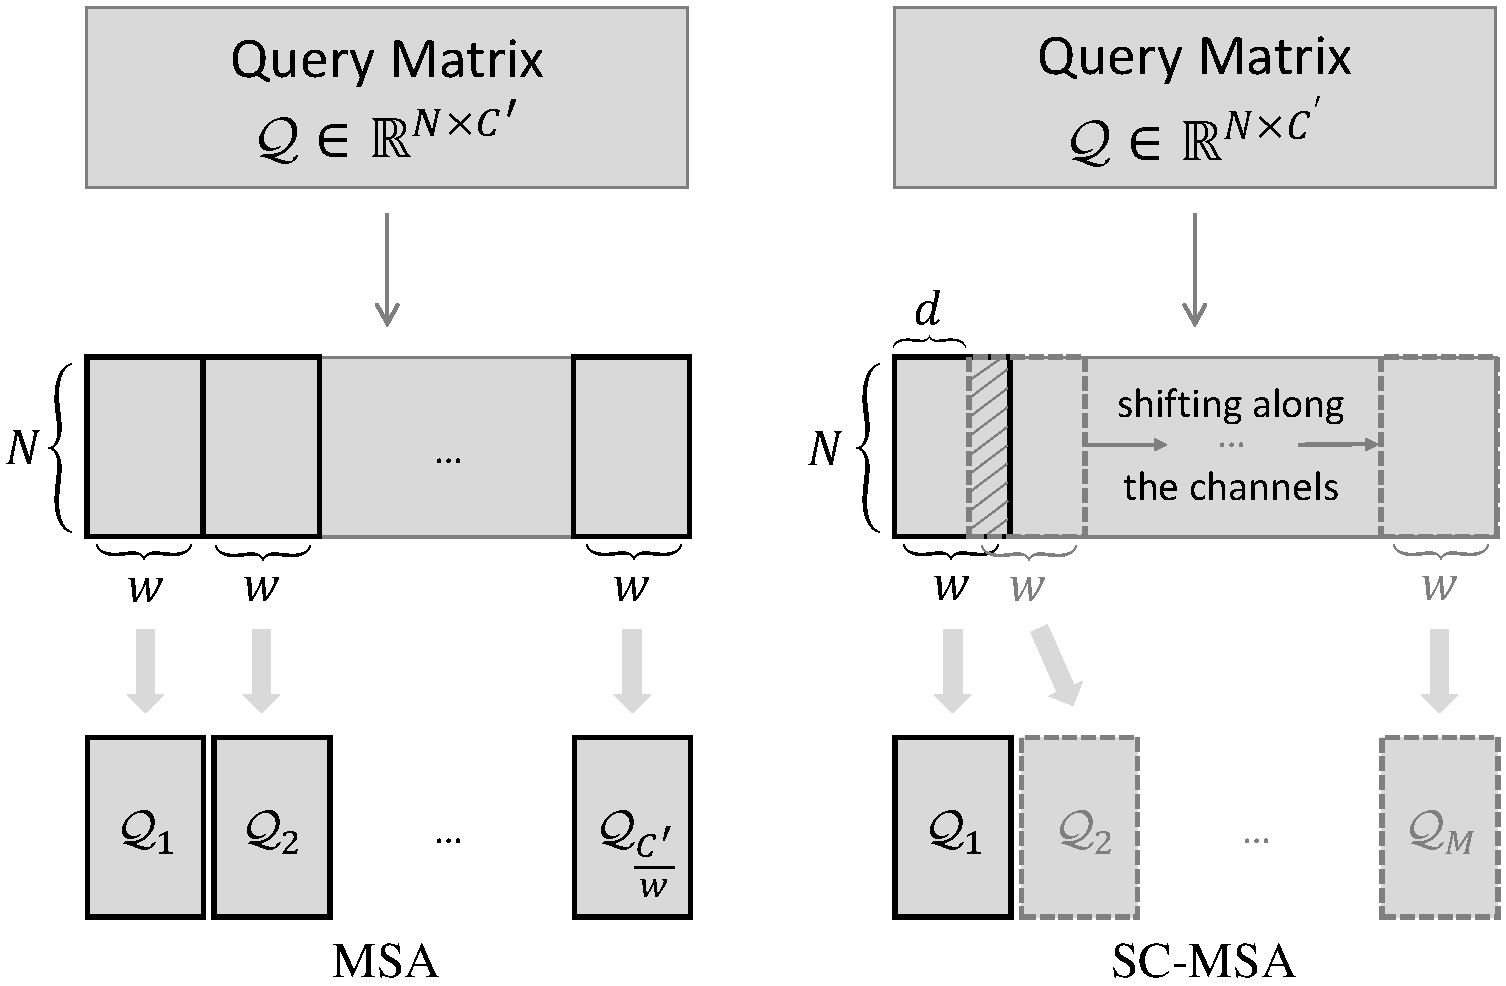
\includegraphics[width=\columnwidth]{images/splits.pdf}
    \captionof{figure}{\small Examples of how regular MSA~\cite{vaswani2017attention} and our SC-MSA generate the low-dimensional splits of query matrix $\mathcal{Q}$ for multi-head processing (the same procedure applies to $\mathcal{K}$ and $\mathcal{V}$).}
    \label{fig:splits}
\end{minipage}
\end{figure}

As Alg.~\ref{alg:msa} states, at first, we apply linear layers (denoted as \enquote{$\mathrm{Linear}$}, and implement as a $1\times1$ convolution) to encode the query matrix $\mathcal{Q}$, key matrix $\mathcal{K}$, and value matrix $\mathcal{V}$. Then, we generate low-dimensional splits of $\mathcal{Q}_m,\mathcal{K}_m,\mathcal{V}_m$ for each head. Particularly, as shown in Fig.~\ref{fig:splits}, regular MSA generates the \emph{independent} splits for the self-attention calculation in corresponding heads. In contrast, our SC-MSA applies a window (dashed square) shift along the channels to ensure that any two consecutive splits have an overlap of $(w-d)$ channels (slashed area), where $w$ is the channel dimension of each split and $d$ represents the channel-wise shift interval each time. After generating the $\mathcal{Q}_m,\mathcal{K}_m,\mathcal{V}_m$ for each head in the mentioned manner, we employ self-attention (Alg.~\ref{alg:msa} steps 8-9) to estimate the point-wise dependencies as the output $\mathcal{O}_m$ of each head. Considering the fact that any two consecutive heads have part of the input in common (\ie, the overlap channels), thus the connections between the outputs $\{\mathcal{O}_1, \mathcal{O}_2, ..., \mathcal{O}_M\}$ (Alg.~\ref{alg:msa} step 11) of multiple heads are established. There are two major benefits of such connections: (i) it is easier to integrate the information between the \emph{connected} multi-head outputs (Alg.~\ref{alg:msa} step 12), compared to using the \emph{independent} multi-head results of regular MSA; and (ii) as the overlapping context is captured from the channel dimension, our SC-MSA can further enhance the channel-wise relations in the final output $\mathcal{O}$, better fulfilling an efficient and effective shuffling-based upsampling strategy than only using regular MSA's point-wise information. These benefits contribute to a faster training convergence and a better upsampling performance, especially when we deploy fewer Transformer Encoders. More practical evidence is provided in the supplementary material.  

It is worth noting that SC-MSA requires the shift interval to be smaller than the channel-wise width of each split (\ie, $d<w$ as in Alg.~\ref{alg:msa}) for a shared area between any two consecutive splits. Accordingly, the number of heads in our SC-MSA is higher than regular MSA (\ie, $M > C^{\prime}/w$ in Fig.~\ref{fig:splits}). More implementation detail and the choices of parameters are provided in Sec.~\ref{sec:pu_body}.
